% Chapter Template

\chapter{Performance Analysis and Optimization}

\label{Chapter6}

\lhead{Chapter 6. \emph{Performance Analysis and Optimisation}}
After implementing the new 2D Ewald summation algorithm, the subsequent objective was to identify performance bottlenecks in the program, as the next critical step in guiding further optimization efforts. Intel VTune Profiler was used for this purpose, as it provides detailed insights into the program’s execution by highlighting time-consuming functions, and parallelization inefficiencies.
% \section{Performance Analysis using Intel VTune Profiler}
\section{Baseline Program}
Hotspot analysis of the program was performed to identify computational bottlenecks. The results in Fig.~(\ref{fig:result1vtune}), indicate that the real-space component accounts for approximately 60-65\% of the total CPU time. The most expensive function was \texttt{dist}, responsible for inter-particle distance calculations, consuming around 25\% of the execution time. This cost is compounded by repeated calls to the \texttt{\_\_erfc} function from \texttt{libm-2.31.so}, contributing approximately 20\% of the total runtime. These findings highlight the need to optimize the real-space calculations, particularly the error function evaluation, to improve overall performance.
% \begin{figure}[htbp]
\begin{figure}[H]
    \centering
    \begin{minipage}{0.7\textwidth}
        \fbox{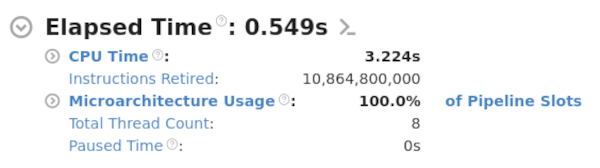
\includegraphics[width=\linewidth]{images/VTuneInitialTime.png}}
    \end{minipage}%
    \begin{minipage}{0.3\textwidth}
        \caption{Execution time details for baseline program.}
    \end{minipage}
\end{figure}
% \begin{figure}[htbp]
\begin{figure}[H]
    \centering
    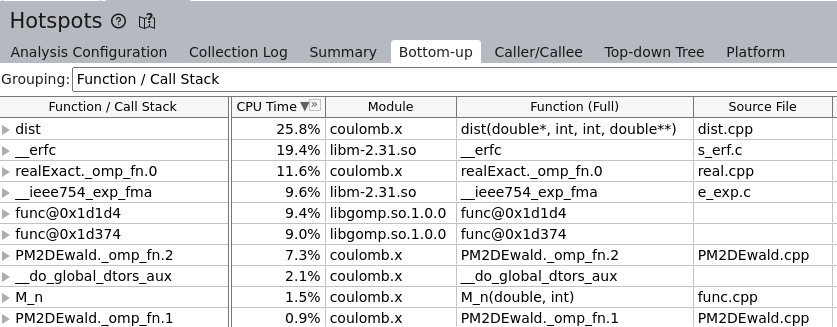
\includegraphics[width = \linewidth]{images/VTuneInitialHotspot.png}
    \caption{Hotspot analysis of the baseline Ewald summation implementation, as reported by Intel VTune Profiler. A significant portion of total CPU time is concentrated in the \textit{dist} function (25.8\%), the standard math library's \textit{\_\_erfc} function (19.4\%).}
    \label{fig:result1vtune}
\end{figure}

\section{Polynomial Interpolation of Error Function}
A significant portion of the program’s execution time was consumed by calls to the \verb|std::erfc| function. To reduce the computational cost associated with evaluating the complementary error function \(\operatorname{erfc}(x)\) in the real-space part of the Ewald summation, a polynomial interpolation approach was adopted. This technique is outlined in \textit{Handbook of Mathematical Functions by Abramowitz and Stegun (1964)}. The expression used is
\begin{equation}  
    erf(x) = 1 - (a_1 t + a_2 t^2 + a_3 t^3 + a_4 t^4 + a_5 t^5) e^{-x^2} + \epsilon(x)
\end{equation}
\[
    t = \frac{1}{1 + px}, \quad |\epsilon(x)| \leq 1.5 \times 10^{-7},
\]
\[
p = 0.3275911, \\
a_1 = 0.254829592, \\
a_2 = -0.284496736,
\]
\[
a_3 = 1.421413741, \\
a_4 = -1.453152027, \\
a_5 = 1.061405429.
\]This polynomial was then used as a direct replacement for the standard \(\operatorname{erfc}(x)\) function within the real-space evaluation.
\section{Additional Optimizations}
\subsection{Array Flattening}
In the implementation, data involving multiple dimensions must be stored in several parts of the program, such as atom positions and charge spreading array for the SPME. While multidimensional arrays are a natural choice for such data, they have drawbacks. 

Dynamically allocated multidimensional arrays often lead to scattered memory layouts and multiple pointer dereferences. This results in poor cache performance and added complexity in memory management. 
To address this, a one-dimensional array was used to represent the multidimensional structure. For an array with rank $d$ and dimensions $n_1\times \ldots \times n_d$, an element at ($i_1\times \ldots \times i_d$) maps to:
\begin{flalign*}
    i_d + n_d \cdot \left( i_{d-1} + n_{d-1} \cdot \left( \ldots + n_2 \cdot i_1 \right)\right)
\end{flalign*}
This approach reduced overhead, improved memory locality, and allowed faster access through direct indexing.
\subsection{Vectorization}
Vectorization enables the simultaneous processing of multiple data elements using a single instruction. This approach significantly improves both the speed and efficiency of computations. It is a fundamental technique in high-performance numerical computing, scientific simulations, graphics, and machine learning, as it leverages the SIMD (Single Instruction Multiple Data) capabilities present in modern processors.

In this work, the program has been compiled using the flags \texttt{-O3}, \texttt{-mavx2}, \texttt{-march=native}, \texttt{-ftree-vectorize}, and \texttt{-ftree-vectorizer-verbose=1}. The \texttt{-O3} flag enables aggressive optimization, including automatic vectorization of loops. The \texttt{-mavx2} flag ensures that the generated code utilizes AVX2 instructions, which operate on 256-bit registers. This allows the simultaneous processing of 8 single-precision floating-point numbers or 4 double-precision floating-point numbers, thereby greatly accelerating loops and computation-intensive sections of the code.
\section{Performance of Optimized Implementation}
Following the improvements, hotspot analysis of the optimized implementation Fig.~(\ref{fig:resultVTuneFinal}), shows a notable shift in the computational profile. The \texttt{\_\_erfc} function no longer appears among the major hotspots. The primary contributors to CPU time are now \texttt{dist} (35.4\%) and \texttt{real\_omp\_fn.0} (23.2\%), both associated with real-space computations. 
% Detailed performance improvements are presented in the \textit{Numerical Analysis} section of the thesis.
\begin{figure}[htbp]
% \begin{figure}[]
    \centering
    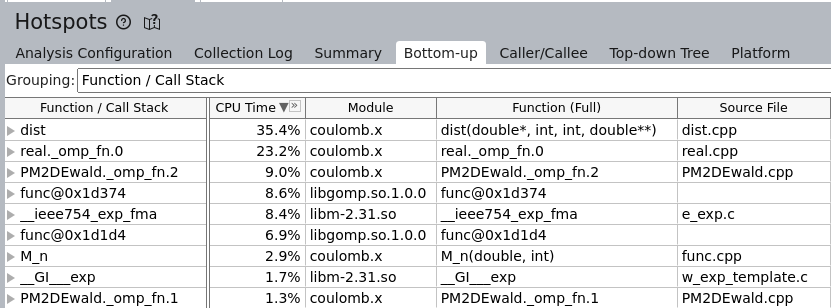
\includegraphics[width = \linewidth]{images/VTuneFinalHotSpots.png}
    \caption{Hotspot analysis of the optimized Ewald summation implementation, using a polynomial interpolation for the error function. The overall CPU time distribution indicates improved efficiency in the real-space term.}
    \label{fig:resultVTuneFinal}
\end{figure}
\begin{figure}[htbp]
% \begin{figure}[]
    \centering
    \begin{minipage}{0.7\textwidth}
        \fbox{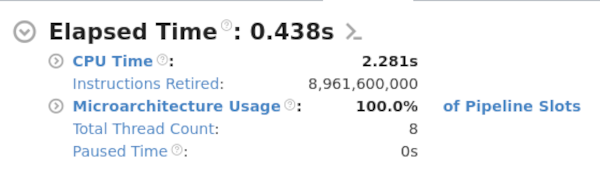
\includegraphics[width=\linewidth]{images/VTuneFinalTime.png}}
    \end{minipage}%
    \begin{minipage}{0.3\textwidth}
        \caption{Execution time details for improved program.}
    \end{minipage}
\end{figure}

\section{Parallelisation}
% \subsubsection*{Real Space}

% \subsubsection*{Reciprocal Space}
\subsection{OpenMP}
OpenMP is a shared-memory parallel programming standard that allows for step-by-step parallelization. It requires only minor changes to the original sequential code, making it easy to apply. Unlike other methods that need a supercomputer, OpenMP can provide speedup even on personal computers with two or more processor cores.
\subsection{Reduction Clauses}
\_\_restrict\_\_

\subsection{Race condition during Charge Spreading for SPME}
A naïve implementation, which uses one thread to map the spread of each individual charge onto the grid, would encounter synchronization problems when different threads attempt to accumulate charge on the same grid location, thus necessitating the use of thread-safe atomic memory operations.

During the computation of the charge spreading array $Q$, the contribution to each grid point is determined by the interpolation weights associated with each particle. In a parallel implementation, multiple threads may attempt to update the same grid point concurrently if the interpolation regions of different particles overlap. This leads to a \textit{race condition}, where the final value at a given grid point depends on the unpredictable timing of memory accesses by different threads. Some contributions may be overwritten or lost entirely without proper synchronization, resulting in incorrect results.

The \verb|atomic update| clause provided by OpenMP was employed to prevent this. It ensures that updates to a shared memory location are performed atomically, preventing simultaneous read/write operations by multiple threads and thereby eliminating the race condition.
\subsection{Implementation Correctness}

% the indexing line is taken from the fftw tutorial website.
% https://www.fftw.org/fftw2_doc/fftw_2.html